\documentclass{article}
\usepackage{iclr2024_conference,times}
\usepackage{amsmath}
\usepackage[utf8]{inputenc}
\usepackage[T1]{fontenc}
\usepackage{xcolor}
\usepackage{hyperref}
\usepackage{url}
\usepackage{booktabs}
\usepackage{tabularx}
\usepackage{xltabular}
\usepackage{array}
\usepackage{microtype}
\usepackage{graphicx}
\usepackage{float}
\usepackage{caption}

\captionsetup{labelsep=period}
\captionsetup[table]{skip=6pt}
\captionsetup[figure]{skip=6pt}
\iclrfinalcopy
\setcitestyle{numbers,square,comma}
\renewcommand{\headrulewidth}{0pt}
\hyphenpenalty=5000
\tolerance=1000
\emergencystretch=2em
\definecolor{ReferenceBlue}{HTML}{0645AD}
\hypersetup{colorlinks=true,urlcolor=ReferenceBlue,citecolor=black,linkcolor=black}

\hypersetup{pdftitle={The Top 100 Web3 Employers Index},pdfauthor={Hashtag Web3}}

\makeatletter
% Professional Whitepaper Header (No subheading, tight publisher block)
\def\@maketitle{\vbox{\hsize\textwidth
\centering
\vskip 0.12in
{\LARGE\bfseries The Top 100 Web3 Employers Index\par}
\vskip 0.14in
{\normalsize\textbf{Hashtag Web3}\\[2pt]
\small\href{https://hashtagweb3.com}{hashtagweb3.com}\par}
\vskip 0.20in}}

% Executive Summary replacing academic Abstract
\renewenvironment{abstract}{%
  \vskip.05in
  \centerline{\large\bfseries Executive Summary}
  \vspace{0.8ex}
  \begin{quote}
}{%
  \par\end{quote}\vskip 1.5ex
}

% Clean bold section titles matching industry whitepapers
\renewcommand\section{\@startsection {section}{1}{\z@}%
  {-2.0ex plus -0.5ex minus -.2ex}%
  {1.1ex plus 0.2ex minus 0.1ex}%
  {\large\bfseries\raggedright}}

\renewcommand\subsection{\@startsection{subsection}{2}{\z@}%
  {-1.6ex plus -0.4ex minus -.2ex}%
  {0.7ex plus .2ex}%
  {\normalsize\bfseries\raggedright}}

\renewcommand\subsubsection{\@startsection{subsubsection}{3}{\z@}%
  {-1.3ex plus -0.3ex minus -.2ex}%
  {0.5ex plus .1ex}%
  {\normalsize\bfseries\raggedright}}

% Ensure single clean numbering with period
\renewcommand{\@seccntformat}[1]{\csname the#1\endcsname.\hspace{0.7em}}
\makeatother

\begin{document}
\raggedbottom
\maketitle

\begin{abstract}
The Top 100 Web3 Employers Index tracks active hiring across one hundred leading organizations in decentralized technology. Published by Hashtag Web3, the ranking uses primary data collected directly from enterprise applicant tracking systems, including Greenhouse, Ashby, and Lever. Traditional directories often charge companies for placement or rely on estimates such as website traffic and venture capital runway. Our index removes all sponsorship fees and synthetic estimates. Companies are evaluated on four verifiable factors, including active job volume, department diversity, remote availability, and salary disclosure. Our data reveals high labor concentration, where the top ten employers account for 34.8 percent of all open positions. Remote work availability averages 39 percent across the index, with software infrastructure reaching 77 percent while quantitative trading desks report 6 percent. This whitepaper explains our qualification standards, scoring formulas, data safeguards, and labor market findings.
\end{abstract}

\section{Executive Overview and the Hashtag Web3 Benchmark}

The Top 100 Web3 Employers Index serves as an open, verifiable benchmark for talent allocation, organizational growth, and workforce research across the decentralized technology ecosystem. Job seekers, founders, researchers, and institutional capital allocators consult employer lists to evaluate organizational stability and labor demand. In rapidly developing industries, reliable workforce data is difficult to gather, and public directories often struggle to maintain independence and accuracy \cite{ref1,ref2}.

Traditional company rankings frequently depend on two questionable practices. First, commercial publishers often charge promotional fees to place or highlight specific brands. Second, aggregators frequently substitute real data with synthetic models, such as inferred traffic volumes, unverified venture funding runway tiers, and small sample surveys. These unverified metrics distort rankings and produce an inaccurate representation of organizational health.

This whitepaper documents the design, mathematical framework, and empirical findings of the Hashtag Web3 Top 100 Employers Index. The index relies entirely on primary hiring data collected directly from enterprise applicant tracking systems, including Greenhouse, Ashby, and Lever \cite{ref1,ref2,ref3}. By discarding speculative metrics, our index establishes a verifiable benchmark of active organizational hiring.

Our automated data pipeline processes active job postings through five distinct stages, from primary ingestion to live publication.

\begin{figure}[H]
\centering
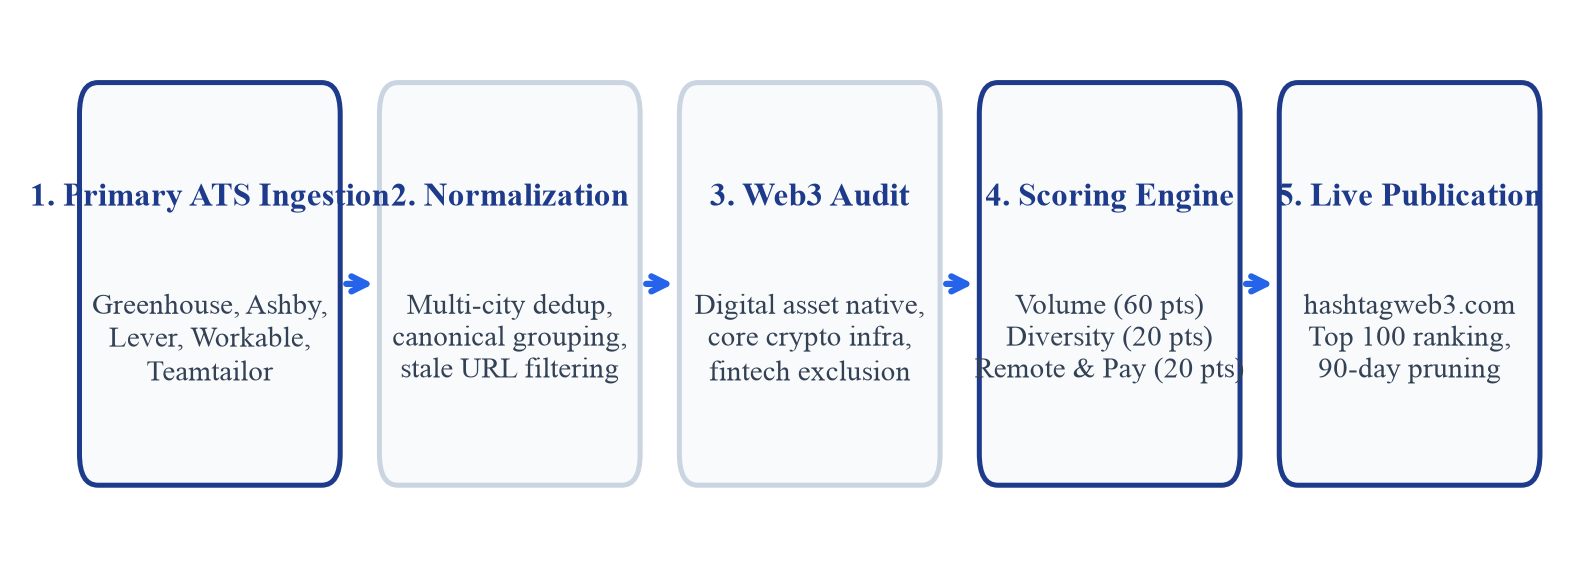
\includegraphics[width=0.98\textwidth]{figure1_pipeline.png}
\caption{The Hashtag Web3 verifiable data pipeline and verification architecture}
\end{figure}

\section{Why Conventional Rankings Fail and Our Anti-Synthetic Principles}

Early iterations of employer ranking algorithms frequently incorporated modeled variables in an attempt to capture qualitative attributes, such as institutional stability, candidate interest, and workplace flexibility. Our analysis indicates that these synthetic variables create systematic distortions when applied to early stage and mid size enterprises.

\subsection{The Single Job Outlier Problem}

In uncalibrated scoring systems, synthetic baseline points can allow an early stage project with only one open position to rank ahead of organizations actively hiring multiple engineering teams. In historical experiments, algorithms frequently assigned credit across three estimated categories.

\begin{enumerate}
\item \textbf{Modeled Financial Runway.} The algorithm estimated cash runway tiers based on external venture capital announcements, awarding up to 25 points.
\item \textbf{Search Intent Estimates.} The algorithm estimated candidate interest from third-party search indexes, awarding up to 15 points.
\item \textbf{Workplace Quality Overrides.} The algorithm awarded full workplace points if a single listing mentioned remote flexibility, contributing up to 20 points.
\end{enumerate}

Under this flawed structure, an early stage project with a single open job could accumulate more than 60 points out of 100. This score exceeded the point totals of established companies with five to ten active technical openings, simply because the larger employers did not carry modeled score boosts.

\begin{figure}[H]
\centering
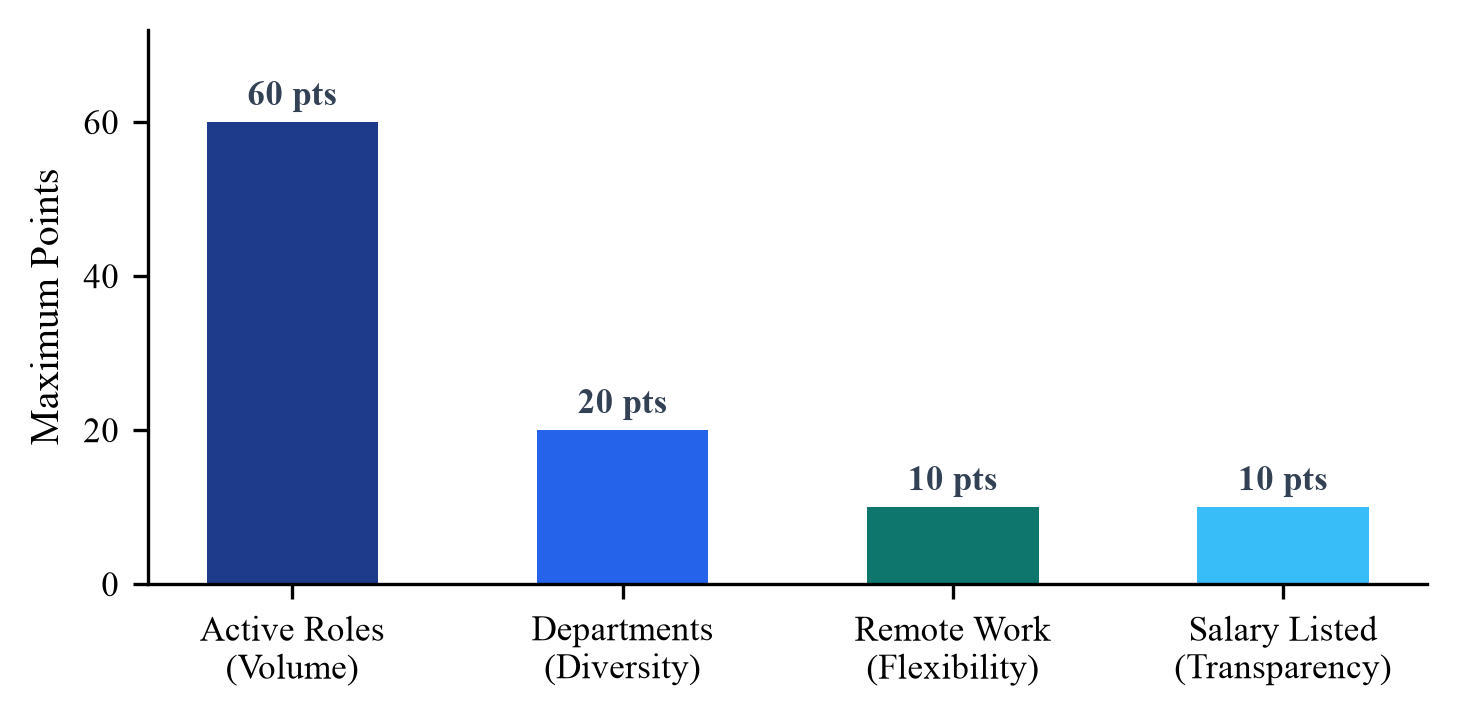
\includegraphics[width=0.88\textwidth]{figure2_points.png}
\caption{Maximum point allocation across the four verified index dimensions}
\end{figure}

\subsection{Eliminating Speculative Variables}

To resolve these distortions, our methodology removes all unverified inputs. We discard estimated funding runways because private equity rounds and token treasury balances are rarely auditable in real time. We eliminate search volume approximations because search traffic frequently reflects media events or market volatility rather than genuine career interest. We also remove manual culture scores, which are vulnerable to sample bias and employer manipulation.

Under our reformed framework, verified hiring capacity serves as the primary evaluation criterion. An employer with a single listing cannot outrank an organization hiring dozens of specialists across diverse teams. In our current dataset, every organization in the top 100 maintains at least two open roles, and 96 employers maintain three or more active positions.

\section{Index Eligibility and Core Web3 Qualification Standards}

A rigorous industry index requires precise boundary definitions. Web3 technology operates at the intersection of cryptography, distributed ledgers, peer to peer networks, and decentralized protocols. Because traditional technology corporations and financial brokerages have established digital asset trading desks or experimental blockchain teams, our index establishes clear qualification standards to maintain sector relevance.

\subsection{Baseline Inclusion Standards}

To qualify for evaluation in the index, an organization must satisfy three baseline conditions.

\begin{enumerate}
\item \textbf{Native Digital Asset Focus.} The core business model, primary product offering, and operational revenue must derive from decentralized networks, digital assets, or cryptographic infrastructure.
\item \textbf{Direct Technical Engagement.} The organization must develop protocols, distributed applications, cryptographic custody software, specialized decentralized finance instruments, security audits, or hardware infrastructure supporting decentralized networks.
\item \textbf{Machine-Verifiable Career Feeds.} The organization must publish career listings through supported enterprise applicant tracking systems, enabling automated verification \cite{ref1,ref2,ref3,ref4,ref5}.
\end{enumerate}

\subsection{Exclusion of Non-Native and Traditional Fintech Entities}

To protect ranking integrity, our index strictly excludes traditional financial technology platforms, corporate spend management companies, and conventional equity brokerages whose core revenue models lie outside decentralized networks.

When we inspect full enterprise hiring feeds from large financial institutions, the overwhelming majority of their open positions involve conventional retail equity execution, corporate credit cards, traditional fiat clearing, and non-crypto enterprise sales.

Including these non-native enterprises would distort the index. An enterprise payment processor with thousands of conventional IT openings would overshadow dedicated decentralized engineering teams, despite dedicating only a minor fraction of its budget to digital assets.

Specific exclusion categories include the following groups.

\begin{enumerate}
\item \textbf{Corporate Spend Management and Commercial Card Platforms.} Enterprises whose primary revenue comes from corporate expense software and commercial charge cards, such as Ramp, are excluded.
\item \textbf{Regulated Retail Broker Dealers.} Registered broker dealers whose primary business involves conventional equity trading APIs, clearing services, and retail securities, such as Alpaca and DriveWealth, are excluded.
\item \textbf{Regulated Traditional Event Contract Markets.} Exchanges operating as traditional contract markets under Commodity Futures Trading Commission regulation for non-crypto binary event contracts, such as Kalshi, are excluded \cite{ref9}.
\item \textbf{Traditional Fiat Payment Processors.} Global payment processors whose main revenue derives from traditional merchant acquiring and card network processing are excluded.
\end{enumerate}

\section{Scoring Methodology and Mathematical Formulation}

The Top 100 Web3 Employers Index evaluates organizations across four distinct, machine-verifiable components. Each component is derived directly from live listings, producing a composite score bounded between zero and one hundred points.

\begin{table}[H]
\centering
\caption{Mathematical weighting and target dimension summary}
\footnotesize
\begin{tabularx}{\textwidth}{@{}>{\raggedright\arraybackslash}p{2.2cm}>{\raggedright\arraybackslash}p{2.8cm}>{\raggedright\arraybackslash}p{1.2cm}>{\raggedright\arraybackslash}X@{}}
\toprule
\textbf{Component} & \textbf{Target Dimension} & \textbf{Weight} & \textbf{Mathematical Model} \\
\midrule
Volume ($V_i$) & Active Open Roles & 60\% & Logarithmic scaling relative to top employer \\[3pt]
Diversity ($D_i$) & Functional Breadth & 20\% & Linear progression across up to 10 departments \\[3pt]
Flexibility ($R_i$) & Distributed Access & 10\% & Proportion of positions supporting remote work \\[3pt]
Transparency ($S_i$) & Compensation Openness & 10\% & Proportion of positions with upfront salary ranges \\[3pt]
\bottomrule
\end{tabularx}
\end{table}

\subsection{Component Definitions and Point Weighting}

\textbf{1. Hiring Volume ($V_i$) with 60 Points Maximum.}
Hiring volume reflects total active open roles. To prevent a single mega-employer from compressing all other participants while rewarding genuine capacity, volume is scaled logarithmically relative to the maximum observed employer in the dataset.

Let $J_i$ represent the verified active job count for employer $i$, and let $J_{\max}$ represent the highest observed job count in the snapshot. The volume score is calculated through the following equation.
\[
V_i = 60 \cdot \frac{\ln(1 + J_i)}{\ln(1 + J_{\max})}
\]

In our current dataset, the highest observed volume is Coinbase with 75 verified positions. An employer with 75 jobs receives the full 60 points. An employer with 46 jobs receives 53.3 points. An employer with 24 jobs receives 44.6 points. An employer with 10 jobs receives 33.2 points. An employer with 2 jobs receives 15.2 points. An organization with only 1 job receives 9.6 points.

\begin{figure}[H]
\centering
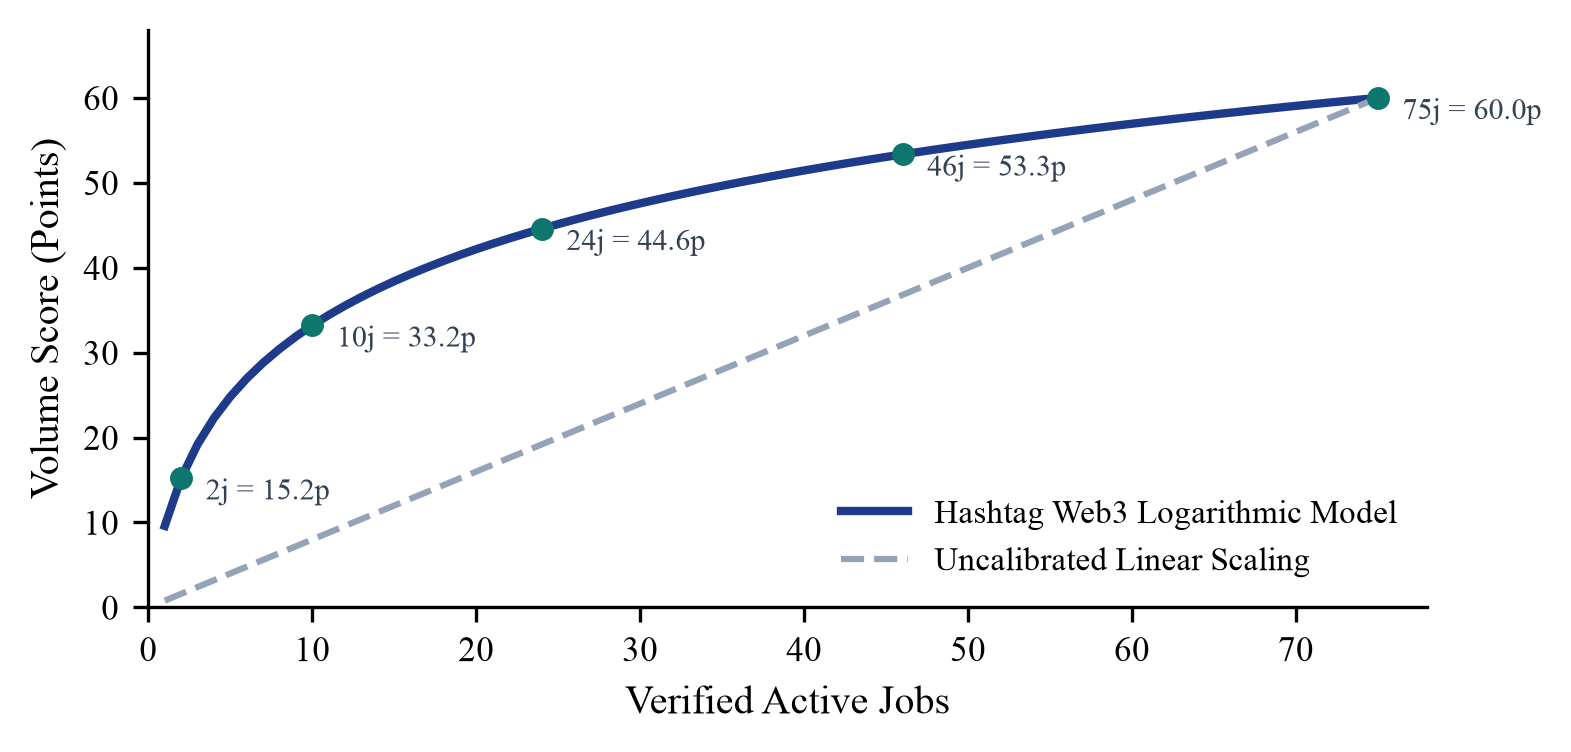
\includegraphics[width=0.88\textwidth]{figure3_curve.png}
\caption{Logarithmic volume scoring curve compared to an uncalibrated linear baseline}
\end{figure}

\textbf{2. Functional Role Diversity ($D_i$) with 20 Points Maximum.}
Role diversity measures whether an organization is hiring across multiple departments or concentrating solely in a single area. We evaluate nine functional categories, including Engineering, Product, Design, Security, Legal, Operations, Marketing, Business Development, and Finance.

Let $K_i$ represent the number of distinct detected departments with open roles at employer $i$. The diversity score is calculated as follows.
\[
D_i = \min(20, \; 2 \cdot K_i)
\]

Organizations hiring across ten or more functional categories achieve the full 20 points.

\textbf{3. Workplace Flexibility and Remote Availability ($R_i$) with 10 Points Maximum.}
Remote availability measures the proportion of open positions accessible to geographically distributed workers. Let $J_{\text{remote}, i}$ represent the number of positions explicitly marked as remote. The remote score is given by the following relationship.
\[
R_i = 10 \cdot \frac{J_{\text{remote}, i}}{J_i}
\]

\textbf{4. Compensation Transparency ($S_i$) with 10 Points Maximum.}
Compensation transparency evaluates the proportion of job listings that provide upfront salary bands. Let $J_{\text{salary}, i}$ represent the number of listings containing verified wage ranges. The salary transparency score is defined by the following expression.
\[
S_i = 10 \cdot \frac{J_{\text{salary}, i}}{J_i}
\]

\subsection{Composite Score Calculation}

The final index score for employer $i$ is the linear sum of the four components.
\[
\text{Score}_i = V_i + D_i + R_i + S_i
\]

\subsection{Ranking Order and Tiebreaker Rules}

To ensure that verified hiring capacity remains the foundation of the index, organizations are ordered primarily by verified active job count.
\[
\text{Rank}(i) \prec \text{Rank}(j) \quad \text{if} \quad J_i > J_j
\]

When two employers maintain identical job counts, the composite score serves as the secondary tiebreaker.
\[
\text{Rank}(i) \prec \text{Rank}(j) \quad \text{if} \quad J_i = J_j \quad \text{and} \quad \text{Score}_i > \text{Score}_j
\]

This hierarchy guarantees that an organization hiring ten engineers will always place above an organization hiring two engineers, regardless of peripheral bonus points.

\section{Key Market Findings Across the Top 100}

Analysis of active openings across our Top 100 reveals several structural characteristics of the decentralized technology labor market.

\begin{figure}[H]
\centering
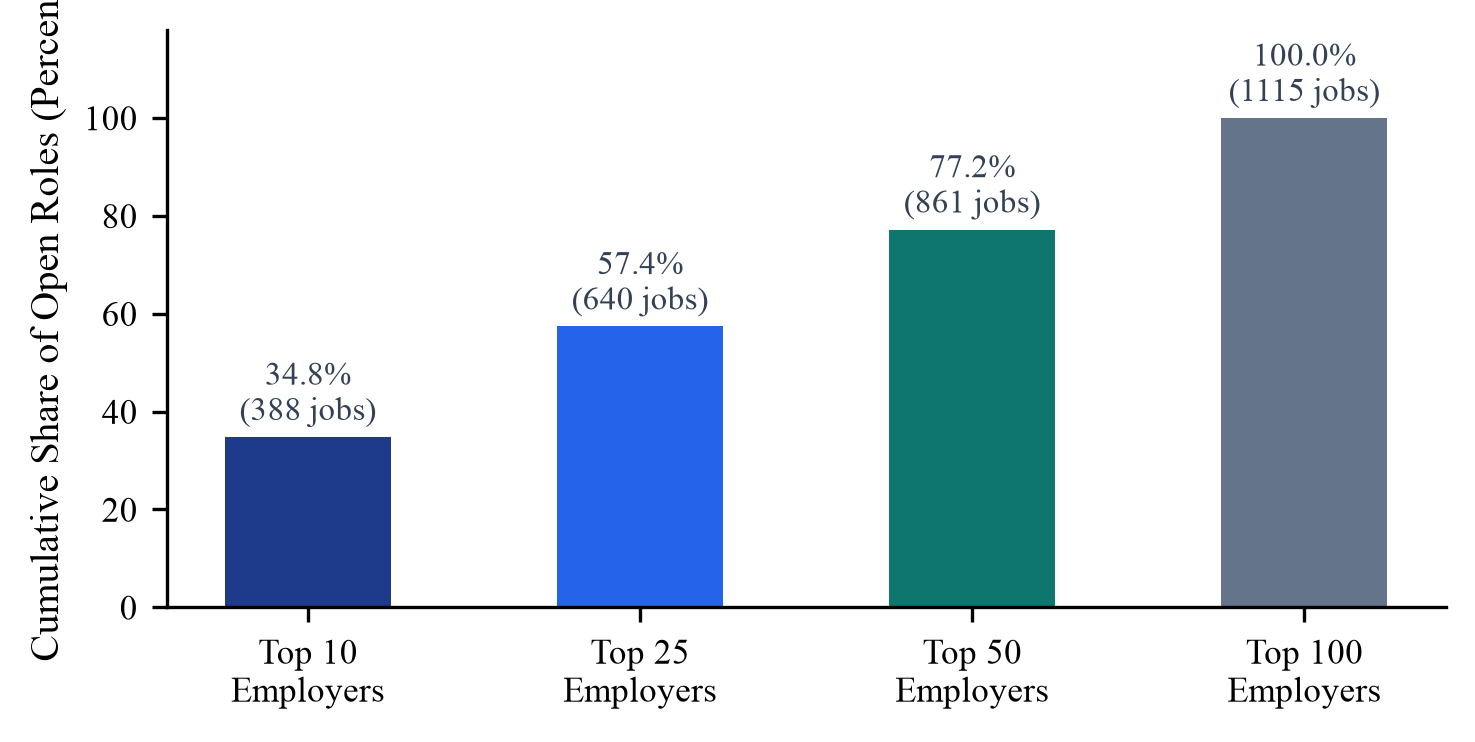
\includegraphics[width=0.88\textwidth]{figure4_concentration.png}
\caption{Cumulative hiring concentration across top employer tiers}
\end{figure}

\subsection{Headcount Concentration Across Top Employers}

Hiring capacity in the Web3 sector exhibits strong power law characteristics. In our sample of 100 employers, the top 10 organizations account for 388 open jobs, representing 34.8 percent of all tracked positions. The top 25 employers account for 640 jobs, representing 57.4 percent of the total. The top 50 employers account for 861 jobs, representing 77.2 percent of the total.

This concentration indicates that large, revenue-generating centralized platforms maintain durable balance sheets capable of supporting extensive expansion through shifting market cycles. Conversely, earlier stage protocol teams and decentralized autonomous organization foundations operate with lean headcounts, typically maintaining between two and seven open positions.

\begin{figure}[H]
\centering
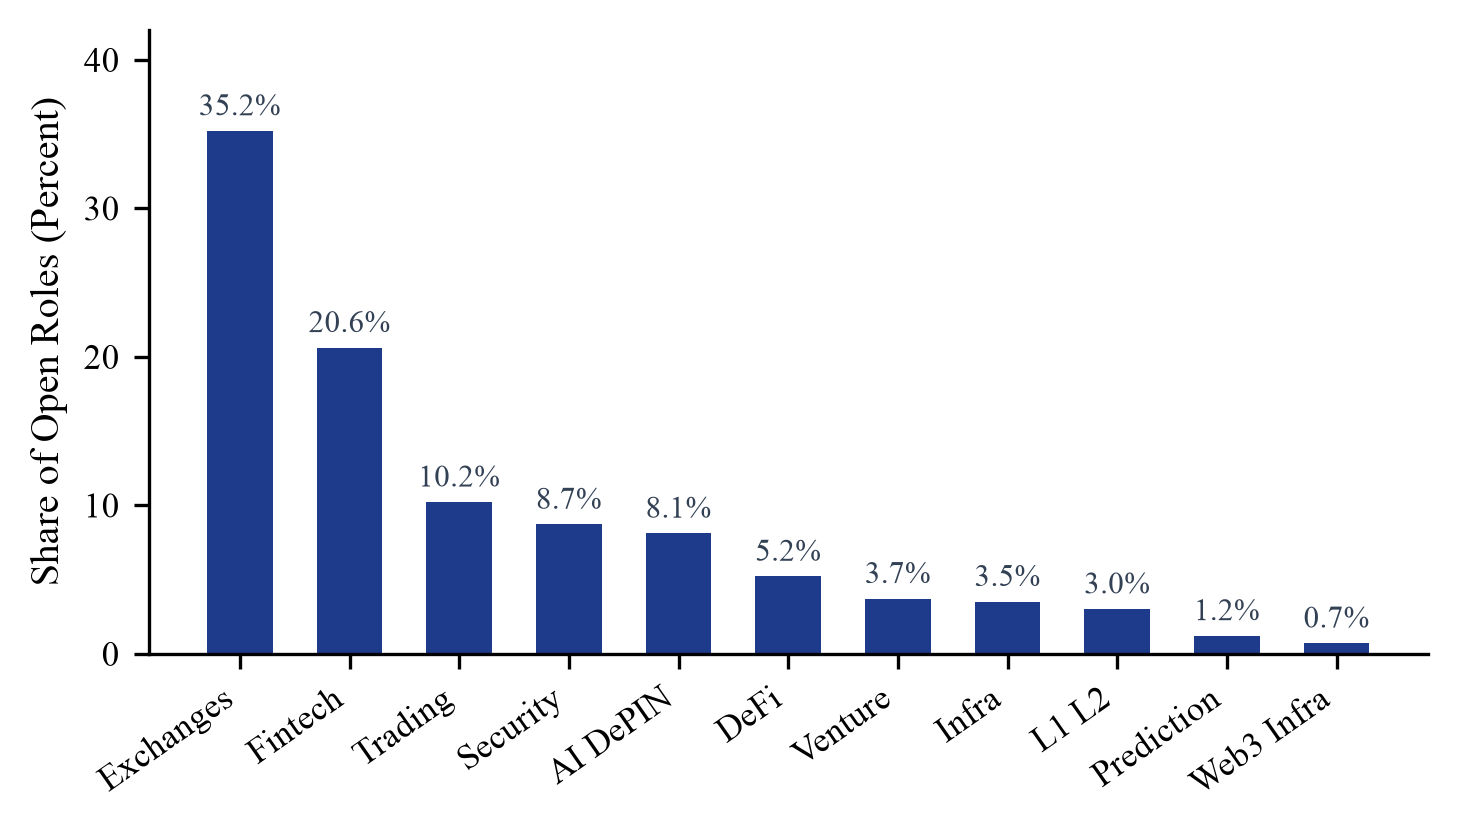
\includegraphics[width=0.88\textwidth]{figure5_sectors.png}
\caption{Share of tracked open positions by industry subsector}
\end{figure}

\subsection{Industry Sector Breakdown}

The 100 employers in the index span 11 functional sectors. Centralized Exchanges and Custody platforms lead all categories, accounting for 392 positions (35.2 percent) across 20 organizations. Fintech and Payments platforms represent the second largest segment, with 230 positions (20.6 percent) across 20 organizations. Quantitative Trading and Market Making firms account for 114 positions (10.2 percent) across 10 organizations.

Emerging categories show notable activity. The Artificial Intelligence and Decentralized Physical Infrastructure Networks sector accounts for 90 positions (8.1 percent) across 8 companies, demonstrating investment at the intersection of distributed compute, cryptographic verification, and machine learning infrastructure.

\section{Workplace Flexibility and Remote Hiring Patterns}

Remote work patterns within the Web3 labor market differ significantly across functional subsectors. Across the entire index of 100 employers, approximately 39 percent of tracked listings are marked as remote.

\begin{figure}[H]
\centering
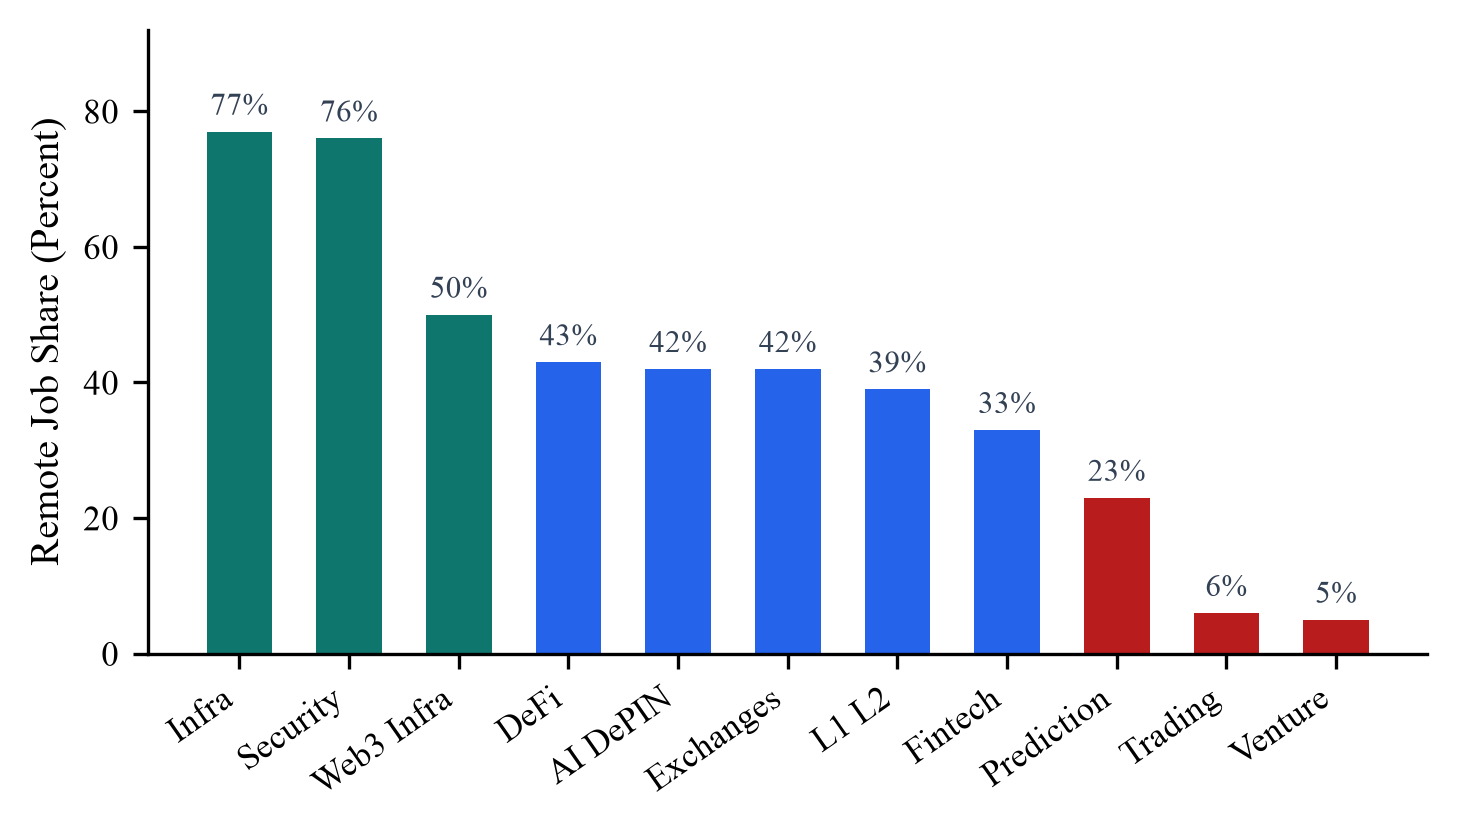
\includegraphics[width=0.88\textwidth]{figure6_remote.png}
\caption{Remote work availability by industry subsector}
\end{figure}

\subsection{Sectors Leading in Distributed Work}

Our data indicates that remote work availability is highest among pure software and protocol engineering teams. Infrastructure and Tooling providers demonstrate a 77 percent remote listing rate, followed by Security and Auditing firms at 76 percent. These organizations frequently coordinate work asynchronously through open source code repositories, automated testing pipelines, and distributed smart contract deployments.

\subsection{Structural Drivers of In-Person Requirements}

In contrast, Quantitative Trading desks report only 6 percent remote availability, and Venture firms report 5 percent remote availability. This low remote prevalence appears to be driven by several operational and regulatory factors.

\begin{enumerate}
\item \textbf{Low Latency Infrastructure.} High frequency digital asset trading firms frequently require personnel to operate in close proximity to physical trading colocation centers and proprietary hardware nodes.
\item \textbf{Market Compliance and Security Controls.} Strict risk management protocols, custody compliance checks, and supervisory rules governing trading desks encourage physical office presence.
\item \textbf{Deal Origination and Partnership Sourcing.} Venture capital and corporate advisory entities continue to prioritize in-person negotiation and regional network density.
\end{enumerate}

\section{Compensation Openness and Regulatory Compliance}

Salary transparency remains an evolving practice within the Web3 sector. Across the index snapshot, approximately 16 to 20 percent of active listings disclose upfront cash compensation ranges.

\subsection{Impact of Statutory Pay Transparency Mandates}

Our geographic analysis indicates that wage disclosure rates are heavily correlated with legal mandates in specific jurisdictions rather than voluntary industry initiatives. In the United States, several states have enacted legislation requiring employers to state wage scales in public postings.

\begin{enumerate}
\item \textbf{California Labor Code Section 432.3.} Enacted under Senate Bill 1162, this statute requires employers with 15 or more workers to disclose the pay scale for any job opening, review, or transfer \cite{ref6}.
\item \textbf{New York Labor Law Section 194-b.} Enacted under Senate Bill S9427A, this law mandates that public listings for positions performing work within New York state publish minimum and maximum salary ranges \cite{ref7}.
\item \textbf{Colorado Revised Statutes Section 8-5-101 et seq.} Enacted under the Equal Pay for Equal Work Act, this legislation requires transparent compensation ranges in any posting accessible to Colorado residents \cite{ref8}.
\end{enumerate}

United States headquartered institutions subject to these regulations exhibit high disclosure rates. In our dataset, Coinbase reports salary ranges on 88 percent of its listings, and Figure reports salary ranges on 77 percent of its listings.

\subsection{Compensation Reporting in Distributed Organizations}

In contrast, offshore protocol foundations, international trading platforms, and decentralized entities frequently exhibit zero percent cash salary disclosure. This opacity is attributable to several factors.

\begin{enumerate}
\item \textbf{Contractor Arrangements.} Many decentralized foundations hire core contributors as independent international contractors rather than conventional domestic employees, placing them outside state labor statutes.
\item \textbf{Token Incentive Compensation.} A substantial portion of total compensation in early stage protocols consists of native token allocations, vest schedules, and governance grants, which are not readily quantified in standard annual base salary fields.
\item \textbf{Jurisdictional Fragmentation.} Operating across multiple legal environments discourages uniform compensation disclosure unless mandated by local authorities.
\end{enumerate}

\section{Subsector Taxonomy and Composition}

To provide granular insight into industry employment, the index organizes qualifying employers into 11 subsectors.

\begin{table}[H]
\centering
\caption{Summary of sector metrics across the top 100 employers}
\footnotesize
\begin{tabularx}{\textwidth}{@{}>{\raggedright\arraybackslash}p{3.0cm}>{\raggedleft\arraybackslash}p{1.0cm}>{\raggedleft\arraybackslash}p{1.1cm}>{\raggedleft\arraybackslash}p{1.2cm}>{\raggedleft\arraybackslash}p{1.1cm}>{\raggedleft\arraybackslash}p{1.0cm}>{\raggedright\arraybackslash}X@{}}
\toprule
\textbf{Sector} & \textbf{Cos} & \textbf{Jobs} & \textbf{Share} & \textbf{Remote} & \textbf{Pay} & \textbf{Top Employer} \\
\midrule
Exchanges and Custody & 20 & 392 & 35.2\% & 42\% & 25\% & Coinbase (75 jobs) \\[2pt]
Fintech and Payments & 20 & 230 & 20.6\% & 33\% & 19\% & Ripple (40 jobs) \\[2pt]
Trading and Quant & 10 & 114 & 10.2\% & 6\% & 23\% & DRW (30 jobs) \\[2pt]
Security and Auditing & 10 & 97 & 8.7\% & 76\% & 14\% & TRM Labs (31 jobs) \\[2pt]
AI and DePIN & 8 & 90 & 8.1\% & 42\% & 3\% & Prime Intellect (24 jobs) \\[2pt]
DeFi Protocols & 13 & 58 & 5.2\% & 43\% & 10\% & Kamino (10 jobs) \\[2pt]
Venture and Research & 3 & 41 & 3.7\% & 5\% & 39\% & Galaxy Digital (25 jobs) \\[2pt]
Infrastructure and Tooling & 7 & 39 & 3.5\% & 77\% & 21\% & Paxos (9 jobs) \\[2pt]
L1 and L2 Protocols & 5 & 33 & 3.0\% & 39\% & 21\% & Mantle Network (12 jobs) \\[2pt]
Prediction Markets & 1 & 13 & 1.2\% & 23\% & 0\% & Polymarket (13 jobs) \\[2pt]
Web3 Infrastructure & 3 & 8 & 0.7\% & 50\% & 0\% & Spruce (3 jobs) \\[2pt]
\bottomrule
\end{tabularx}
\end{table}

\begin{table}[H]
\centering
\caption{Remote work distribution across industry sectors}
\footnotesize
\begin{tabularx}{\textwidth}{@{}>{\raggedleft\arraybackslash}p{0.8cm}>{\raggedright\arraybackslash}p{3.8cm}>{\raggedleft\arraybackslash}p{1.6cm}>{\raggedleft\arraybackslash}p{1.6cm}>{\raggedleft\arraybackslash}X@{}}
\toprule
\textbf{Rank} & \textbf{Sector Name} & \textbf{Tracked Roles} & \textbf{Remote Roles} & \textbf{Remote Availability} \\
\midrule
1 & Infrastructure and Tooling & 39 & 30 & 77\% \\[2pt]
2 & Security and Auditing & 97 & 74 & 76\% \\[2pt]
3 & Web3 Infrastructure & 8 & 4 & 50\% \\[2pt]
4 & DeFi Protocols & 58 & 25 & 43\% \\[2pt]
5 & AI and DePIN & 90 & 38 & 42\% \\[2pt]
6 & Exchanges and Custody & 392 & 165 & 42\% \\[2pt]
7 & L1 and L2 Protocols & 33 & 13 & 39\% \\[2pt]
8 & Fintech and Payments & 230 & 76 & 33\% \\[2pt]
9 & Prediction Markets & 13 & 3 & 23\% \\[2pt]
10 & Trading and Quant & 114 & 7 & 6\% \\[2pt]
11 & Venture and Research & 41 & 2 & 5\% \\[2pt]
\bottomrule
\end{tabularx}
\end{table}

\section{Data Integrity and Verification Safeguards}

A public index based on active hiring must defend against intentional and accidental data distortion. We implement four technical safeguards within our data ingestion pipeline.

\subsection{Real-Time Ingestion and Canonical Deduplication}

Our parser groups listings sharing identical title strings and job specifications into a single canonical posting. Employers frequently cross-list a single position across multiple cities or remote zones to maximize candidate reach. Automated deduplication ensures each distinct open role receives exactly one unit of volume credit.

\subsection{Authenticated Career Domain Verification}

We ingest data only from verified company subdomains on supported enterprise tracking systems. Self-submitted postings, manual employer submissions, and unverified third-party aggregations are rejected.

\subsection{Stale Listing Pruning and Tombstoning}

Any job listing URL that returns an HTTP error or remains unmodified for more than 90 days is marked as inactive and removed from active score calculations. This safeguard ensures that legacy listings do not accumulate unearned score credit.

\subsection{Deterministic Scoring Code}

The scoring calculation is deterministic and transparent. Tiebreaker logic, point weights, and normalization denominators are auditable in code, eliminating manual scoring intervention or subjective editorial bias.

\section{Methodology Boundaries and Ongoing Monitoring}

While our methodology provides verifiable workforce intelligence, several structural boundaries frame the analysis.

\begin{enumerate}
\item \textbf{Enterprise ATS Pipeline Scope.} Organizations utilizing custom internal applicant portals or non-standard hiring software are not indexed by our automated pipeline. Support for additional platforms is added on an ongoing basis.
\item \textbf{Non-Traditional Contributor Workflows.} Web3 organizations frequently recruit specialized contributors through developer bounties, grant programs, and governance proposals without publishing formal job descriptions.
\item \textbf{Token Incentive Structures.} Our compensation metric evaluates cash compensation bands and does not capture equity grants or native token vest schedules. Standardized valuation frameworks for liquid token incentives remain an ongoing research topic.
\end{enumerate}

\section{Complete Index and Top 100 Employers Census}

Table 3 presents the complete empirical census of the one hundred qualifying organizations, ordered by verified active openings and composite score tiebreakers.

\begingroup
\footnotesize
\begin{xltabular}{\textwidth}{@{}>{\raggedleft\arraybackslash}p{0.6cm}>{\raggedright\arraybackslash}p{2.8cm}>{\raggedright\arraybackslash}p{2.9cm}>{\raggedleft\arraybackslash}p{0.7cm}>{\raggedleft\arraybackslash}p{0.7cm}>{\raggedleft\arraybackslash}p{1.0cm}>{\raggedleft\arraybackslash}p{0.8cm}>{\raggedleft\arraybackslash}X@{}}
\caption{Complete empirical census of the top 100 Web3 employers} \label{tab-census} \\
\toprule
\textbf{Rank} & \textbf{Company} & \textbf{Sector} & \textbf{Jobs} & \textbf{Teams} & \textbf{Remote} & \textbf{Pay} & \textbf{Score} \\
\midrule
\endfirsthead
\toprule
\textbf{Rank} & \textbf{Company} & \textbf{Sector} & \textbf{Jobs} & \textbf{Teams} & \textbf{Remote} & \textbf{Pay} & \textbf{Score} \\
\midrule
\endhead
\midrule
\multicolumn{8}{r}{\textit{Continued on next page}} \\
\bottomrule
\endfoot
\bottomrule
\endlastfoot
1 & Coinbase & Exchanges and Custody & 75 & 23 & 83\% & 88\% & 97.1 \\[1.5pt]
2 & OKX & Exchanges and Custody & 73 & 16 & 14\% & 19\% & 82.9 \\[1.5pt]
3 & Bybit & Exchanges and Custody & 47 & 18 & 34\% & 0\% & 77.0 \\[1.5pt]
4 & Kraken & Exchanges and Custody & 46 & 11 & 98\% & 0\% & 83.1 \\[1.5pt]
5 & Ripple & Fintech and Payments & 40 & 12 & 0\% & 45\% & 75.9 \\[1.5pt]
6 & Bitdeer & Exchanges and Custody & 31 & 10 & 13\% & 0\% & 69.3 \\[1.5pt]
7 & TRM Labs & Security and Auditing & 31 & 3 & 100\% & 0\% & 64.0 \\[1.5pt]
8 & DRW & Trading and Quant & 30 & 24 & 0\% & 60\% & 73.6 \\[1.5pt]
9 & Galaxy Digital & Venture and Research & 25 & 9 & 4\% & 24\% & 65.9 \\[1.5pt]
10 & BitGo & Exchanges and Custody & 25 & 9 & 0\% & 12\% & 64.3 \\[1.5pt]
11 & Ajaib Crypto & Trading and Quant & 24 & 8 & 0\% & 0\% & 60.6 \\[1.5pt]
12 & Circle & Fintech and Payments & 24 & 1 & 100\% & 0\% & 56.6 \\[1.5pt]
13 & Prime Intellect & AI and DePIN & 24 & 5 & 0\% & 0\% & 54.6 \\[1.5pt]
14 & Tether & Fintech and Payments & 23 & 7 & 100\% & 0\% & 68.0 \\[1.5pt]
15 & Bitpanda & Exchanges and Custody & 22 & 6 & 0\% & 0\% & 55.4 \\[1.5pt]
16 & Chainalysis & Security and Auditing & 21 & 4 & 90\% & 0\% & 59.8 \\[1.5pt]
17 & Crypto.com & Exchanges and Custody & 21 & 6 & 0\% & 33\% & 58.1 \\[1.5pt]
18 & BVNK & Fintech and Payments & 18 & 6 & 0\% & 56\% & 58.4 \\[1.5pt]
19 & Riot Platforms & AI and DePIN & 16 & 7 & 63\% & 0\% & 59.6 \\[1.5pt]
20 & GoMining & AI and DePIN & 16 & 5 & 94\% & 0\% & 58.7 \\[1.5pt]
21 & StraitsX & Fintech and Payments & 16 & 7 & 0\% & 0\% & 53.3 \\[1.5pt]
22 & Sardine & Fintech and Payments & 15 & 9 & 87\% & 0\% & 65.1 \\[1.5pt]
23 & Figure & Fintech and Payments & 13 & 8 & 46\% & 77\% & 64.9 \\[1.5pt]
24 & Polymarket & Prediction Markets & 13 & 5 & 23\% & 0\% & 48.9 \\[1.5pt]
25 & Chainlink Labs & AI and DePIN & 12 & 5 & 100\% & 0\% & 55.5 \\[1.5pt]
26 & a16z crypto & Venture and Research & 12 & 5 & 8\% & 83\% & 54.6 \\[1.5pt]
27 & Flow Traders & Trading and Quant & 12 & 6 & 0\% & 8\% & 48.3 \\[1.5pt]
28 & Mantle Network & L1 and L2 Protocols & 12 & 5 & 8\% & 0\% & 46.3 \\[1.5pt]
29 & Hut 8 & AI and DePIN & 11 & 6 & 0\% & 0\% & 46.4 \\[1.5pt]
30 & Blockchain.com & Fintech and Payments & 11 & 5 & 0\% & 0\% & 44.4 \\[1.5pt]
31 & Kamino & DeFi Protocols & 10 & 8 & 30\% & 50\% & 57.2 \\[1.5pt]
32 & Flowdesk & Trading and Quant & 10 & 7 & 0\% & 0\% & 47.2 \\[1.5pt]
33 & Jane Street & Trading and Quant & 10 & 7 & 0\% & 0\% & 47.2 \\[1.5pt]
34 & Mesh & Security and Auditing & 9 & 2 & 67\% & 89\% & 51.5 \\[1.5pt]
35 & Zero Hash & Exchanges and Custody & 9 & 4 & 100\% & 0\% & 49.9 \\[1.5pt]
36 & Paxos & Infrastructure and Tooling & 9 & 4 & 89\% & 0\% & 48.8 \\[1.5pt]
37 & Story Protocol & L1 and L2 Protocols & 8 & 3 & 13\% & 88\% & 46.5 \\[1.5pt]
38 & MoonPay & Fintech and Payments & 8 & 6 & 13\% & 0\% & 43.7 \\[1.5pt]
39 & DV Trading & Trading and Quant & 8 & 4 & 13\% & 38\% & 43.5 \\[1.5pt]
40 & Unlimit & Fintech and Payments & 8 & 6 & 0\% & 0\% & 42.4 \\[1.5pt]
41 & Rain & Fintech and Payments & 8 & 3 & 50\% & 0\% & 41.4 \\[1.5pt]
42 & Elliptic & Security and Auditing & 7 & 5 & 100\% & 0\% & 48.8 \\[1.5pt]
43 & Talos & Security and Auditing & 7 & 6 & 57\% & 0\% & 46.5 \\[1.5pt]
44 & Alchemy & Infrastructure and Tooling & 7 & 3 & 100\% & 0\% & 44.8 \\[1.5pt]
45 & Ondo Finance & DeFi Protocols & 7 & 4 & 71\% & 0\% & 43.9 \\[1.5pt]
46 & Aspora & Fintech and Payments & 7 & 5 & 29\% & 0\% & 41.7 \\[1.5pt]
47 & Augustus & Fintech and Payments & 7 & 5 & 0\% & 0\% & 38.8 \\[1.5pt]
48 & Coinflow & Fintech and Payments & 7 & 5 & 0\% & 0\% & 38.8 \\[1.5pt]
49 & Fireblocks & Infrastructure and Tooling & 7 & 1 & 0\% & 43\% & 35.1 \\[1.5pt]
50 & Solflare & DeFi Protocols & 7 & 3 & 0\% & 0\% & 34.8 \\[1.5pt]
51 & Infosys & Security and Auditing & 7 & 1 & 0\% & 0\% & 30.8 \\[1.5pt]
52 & Consensys & Infrastructure and Tooling & 6 & 3 & 100\% & 50\% & 48.0 \\[1.5pt]
53 & HIFI & Fintech and Payments & 6 & 5 & 0\% & 100\% & 47.0 \\[1.5pt]
54 & GRVT & Trading and Quant & 6 & 3 & 100\% & 0\% & 43.0 \\[1.5pt]
55 & SwissBorg & Exchanges and Custody & 6 & 3 & 67\% & 0\% & 39.7 \\[1.5pt]
56 & FalconX & Trading and Quant & 6 & 3 & 0\% & 67\% & 39.7 \\[1.5pt]
57 & Stellar & L1 and L2 Protocols & 6 & 3 & 67\% & 0\% & 39.7 \\[1.5pt]
58 & BitOasis & Exchanges and Custody & 5 & 4 & 0\% & 100\% & 42.8 \\[1.5pt]
59 & Anchorage Digital & Infrastructure and Tooling & 5 & 4 & 100\% & 0\% & 42.8 \\[1.5pt]
60 & Phantom & Exchanges and Custody & 5 & 3 & 100\% & 0\% & 40.8 \\[1.5pt]
61 & Bitvavo & Exchanges and Custody & 5 & 4 & 20\% & 0\% & 34.8 \\[1.5pt]
62 & ComplyAdvantage & Security and Auditing & 5 & 2 & 0\% & 60\% & 34.8 \\[1.5pt]
63 & Breeze Cash & Fintech and Payments & 5 & 3 & 0\% & 0\% & 30.8 \\[1.5pt]
64 & Nexo & Fintech and Payments & 5 & 2 & 20\% & 0\% & 30.8 \\[1.5pt]
65 & Spiko & DeFi Protocols & 5 & 2 & 0\% & 0\% & 28.8 \\[1.5pt]
66 & Newton & Exchanges and Custody & 4 & 3 & 100\% & 0\% & 38.3 \\[1.5pt]
67 & CertiK & Security and Auditing & 4 & 3 & 100\% & 0\% & 38.3 \\[1.5pt]
68 & Morpho & DeFi Protocols & 4 & 3 & 100\% & 0\% & 38.3 \\[1.5pt]
69 & Mysten Labs & L1 and L2 Protocols & 4 & 3 & 100\% & 0\% & 38.3 \\[1.5pt]
70 & Uniswap Labs & DeFi Protocols & 4 & 4 & 75\% & 0\% & 37.8 \\[1.5pt]
71 & Liminal & Exchanges and Custody & 4 & 4 & 25\% & 0\% & 32.8 \\[1.5pt]
72 & Luxor Technology & AI and DePIN & 4 & 2 & 25\% & 0\% & 28.8 \\[1.5pt]
73 & Aave Labs & DeFi Protocols & 4 & 3 & 0\% & 0\% & 28.3 \\[1.5pt]
74 & Baton Corporation & Trading and Quant & 4 & 1 & 0\% & 0\% & 24.3 \\[1.5pt]
75 & Brevan Howard & Venture and Research & 4 & 1 & 0\% & 0\% & 24.3 \\[1.5pt]
76 & Keyrock & Trading and Quant & 4 & 1 & 0\% & 0\% & 24.3 \\[1.5pt]
77 & Pluralis Research & AI and DePIN & 4 & 1 & 0\% & 0\% & 24.3 \\[1.5pt]
78 & Helius & Infrastructure and Tooling & 3 & 3 & 100\% & 0\% & 35.2 \\[1.5pt]
79 & Notabene & Security and Auditing & 3 & 3 & 100\% & 0\% & 35.2 \\[1.5pt]
80 & Digital Asset & AI and DePIN & 3 & 2 & 0\% & 100\% & 33.2 \\[1.5pt]
81 & Polygon Labs & L1 and L2 Protocols & 3 & 2 & 100\% & 0\% & 33.2 \\[1.5pt]
82 & 0x & DeFi Protocols & 3 & 2 & 100\% & 0\% & 33.2 \\[1.5pt]
83 & Groma & Security and Auditing & 3 & 2 & 0\% & 100\% & 33.2 \\[1.5pt]
84 & Orderly Network & DeFi Protocols & 3 & 1 & 100\% & 0\% & 31.2 \\[1.5pt]
85 & Spruce & Web3 Infrastructure & 3 & 2 & 67\% & 0\% & 29.9 \\[1.5pt]
86 & Rhino.fi & DeFi Protocols & 3 & 3 & 33\% & 0\% & 28.5 \\[1.5pt]
87 & Open Standard & Fintech and Payments & 3 & 3 & 33\% & 0\% & 28.5 \\[1.5pt]
88 & 1inch & DeFi Protocols & 3 & 3 & 33\% & 0\% & 28.5 \\[1.5pt]
89 & Coins.ph & Exchanges and Custody & 3 & 3 & 0\% & 0\% & 25.2 \\[1.5pt]
90 & Coinhako & Exchanges and Custody & 3 & 3 & 0\% & 0\% & 25.2 \\[1.5pt]
91 & Lightspark & Exchanges and Custody & 3 & 2 & 0\% & 0\% & 23.2 \\[1.5pt]
92 & ether.fi & DeFi Protocols & 3 & 2 & 0\% & 0\% & 23.2 \\[1.5pt]
93 & Kast & Fintech and Payments & 3 & 2 & 0\% & 0\% & 23.2 \\[1.5pt]
94 & CoinDesk & Web3 Infrastructure & 3 & 1 & 0\% & 0\% & 21.2 \\[1.5pt]
95 & Bullish & Exchanges and Custody & 3 & 1 & 0\% & 0\% & 21.2 \\[1.5pt]
96 & Fasset & Fintech and Payments & 3 & 1 & 0\% & 0\% & 21.2 \\[1.5pt]
97 & Shakepay & Exchanges and Custody & 2 & 1 & 100\% & 100\% & 37.2 \\[1.5pt]
98 & Turnkey & Infrastructure and Tooling & 2 & 2 & 50\% & 100\% & 34.2 \\[1.5pt]
99 & Gauntlet & DeFi Protocols & 2 & 1 & 100\% & 50\% & 32.2 \\[1.5pt]
100 & CoinPoker & Web3 Infrastructure & 2 & 2 & 100\% & 0\% & 29.2 \\[1.5pt]
\end{xltabular}
\endgroup

\clearpage
\begingroup
\small
\renewcommand{\refname}{Data Sources and Regulatory References}
\begin{thebibliography}{99}
\raggedright

\bibitem{ref1}
Greenhouse Software Inc. ``Greenhouse Job Board Specifications and Public API Documentation.'' Technical platform specifications. \href{https://developers.greenhouse.io}{developers.greenhouse.io}.

\bibitem{ref2}
Ashby Inc. ``Ashby Public Career Architecture and API Reference.'' Technical platform documentation. \href{https://developers.ashbyhq.com}{developers.ashbyhq.com}.

\bibitem{ref3}
Lever Inc. ``Lever Postings System Reference and Data Model.'' Technical specifications. \href{https://hire.lever.co}{hire.lever.co}.

\bibitem{ref4}
Workable Software Limited. ``Workable Public Career API Specifications.'' Technical platform reference. \href{https://workable.com}{workable.com}.

\bibitem{ref5}
Teamtailor AB. ``Teamtailor Career Platform Technical Reference.'' Public API documentation. \href{https://teamtailor.com}{teamtailor.com}.

\bibitem{ref6}
California State Legislature. ``Senate Bill 1162, California Labor Code Section 432.3.'' Enacted 2022. Statutory text reproduced by California Legislative Information. \href{https://leginfo.legislature.ca.gov}{leginfo.legislature.ca.gov}.

\bibitem{ref7}
New York State Legislature. ``Senate Bill S9427A, New York Labor Law Section 194-b.'' Enacted 2023. Statutory text reproduced by New York State Senate. \href{https://nysenate.gov}{nysenate.gov}.

\bibitem{ref8}
Colorado General Assembly. ``Senate Bill 19-085, Equal Pay for Equal Work Act, Colorado Revised Statutes Section 8-5-101 et seq.'' Enacted 2021. Statutory text reproduced by Colorado General Assembly. \href{https://leg.colorado.gov}{leg.colorado.gov}.

\bibitem{ref9}
Commodity Futures Trading Commission. ``Order of Registration for KalshiEX LLC as a Designated Contract Market.'' Regulatory filing, November 2020. Public disclosure text reproduced by CFTC. \href{https://cftc.gov}{cftc.gov}.

\end{thebibliography}
\endgroup

\end{document}
